\documentclass{article}
\usepackage[utf8]{inputenc}

\title{Week 10 Lecture 2}
\author{Jared Brannan }

\usepackage{natbib}
\usepackage{graphicx}
\graphicspath{ {./figures/} }
\usepackage{mathtools}
\usepackage{amsthm}
\usepackage{amsmath}
\usepackage{amssymb}
\usepackage{xcolor}
\usepackage{bbm}
\usepackage{bm}
\usepackage{physics}

% indent first line
\usepackage{indentfirst}
% one inch margins
\usepackage[margin=1.0in]{geometry}

\theoremstyle{definition}

\newcommand{\upRiemannint}[2]{
\overline{\int_{#1}^{#2}}
}
\newcommand{\loRiemannint}[2]{
\underline{\int_{#1}^{#2}}
}

\newtheorem{definition}{Definition}
\newtheorem{asside}{Asside}
\newtheorem{conjecture}{Conjecture}
\newtheorem{example}{Example}
\newtheorem{theorem}{Theorem}
\newtheorem{lemma}{Lemma}
\newtheorem{puzzle}{Puzzle}
\newtheorem{corollary}{Corollary}
\newtheorem{proposition}{Proposition}


\begin{document}
\maketitle

\section{Administrative drivel}
\begin{itemize}
	\item
\end{itemize}

\section{Defence and repair -- immune system}
\begin{itemize}
	\item Allergic reaction
		\begin{itemize}
			\item \textbf{Overactive} inflammatory response
				\begin{itemize}
					\item Usually an `innapropriat' response, when no response is really needed.
				\end{itemize}
			\item Hay fever == inflamed sinuses
			\item Hives == inflamed skin
			\item an allergic reaction is a reaction to something that is \textbf{not threatening} 
			\item These are usually treated with an antihistamine, to counteract the histamines that trigger the inflamation response
		\end{itemize}
	\item Also
		\begin{itemize}
			\item General responses to viral invasion
		\end{itemize}
	\item Example -- generalized viral defense (innate)
		\begin{itemize}
			\item Virus-infected cells release \textit{interferons} when they think they're infected by a virus
				\begin{itemize}
					\item Viruses use the cell's $DNA\to RNA\to protein$ machinery to make more viruses.
					\item Viruses lack the tools to reproduce without doing this
					\item After copying their RNA for a while, the cell will burst
				\end{itemize}
			\item Neighboring cells (uninfected) pick up this signal and destroy RNA and reduce protein synthesis
			\item Neighboring cells (infected pick up this signal, and kill themselves (called apoptosis)
			\item This signal also activates the immuce cells (usually T cells) -- at this stage it's a specific response (adaptive)
		\end{itemize}
\end{itemize}
\subsection{Acquired Immunity}
\begin{itemize}
	\item Specific defence against a specific enemy -- 3rd line of defense
		\begin{itemize}
			\item Recognition of a \underline{unique} invader
			\item Not just which \textbf{speecies}  of invader, but which \textit{strain} 
		\end{itemize}
	\item Two responses to infection
		\begin{itemize}
			\item  General responses
				\begin{itemize}
					\item note -- macrophages don't care what kind of bacteria they're killing
				\end{itemize}
			\item specific -- acquired immunity
		\end{itemize}
	\item Steps:
		\begin{itemize}
			\item Find, recognize, and deestroy \textbf{specific} invaders
			\item \textbf{memory} of previous invaders
				\begin{itemize}
					\item allows for faster response to future infections of the same type
				\end{itemize}
			\item Gets a \textbf{wake up call} from innate/general response
		\end{itemize}
	\item Specific immune respons:
		\begin{itemize}
			\item ADA 3rd line of defense
			\item AKA Acquired, Adaptive, or Learned immunity
			\item \underline{Important Terms}:
				\begin{itemize}
					\item \textbf{Pathogen}  == infectious agent (e.g. bacterium)
					\item \textbf{Antigen}  == surface proteins found on all cells -- identifying protien mentioned before
					\item \textbf{Antibody}  == protein produced by immune cell, used to recognize foreign or self antigens
					\item \textbf{antibiotic}  == bacteria-killing drug
						\begin{itemize}
							\item Only work on prokareotes (bacteria, etc. ring DNA which is silly), not on eukareotes (mamals, trees, etc. thinggs with nuclei)
							\item chemicals that kill eukareotes tend to also kill the host -- no good
						\end{itemize}
				\end{itemize}
		\end{itemize}
	\item Antigen/antibodies
		\begin{itemize}
			\item The antibodies identify antigens by their shape
				\begin{itemize}
					\item They bind to the antigen and this labels the cell for distruction
				\end{itemize}
			\item antibodies can bind to 2+ antigens, allowing them to group cells together
				\begin{center}
					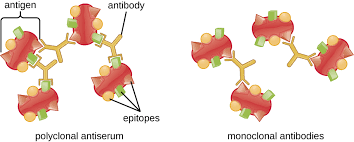
\includegraphics[width=30em]{antibody}
				\end{center}
		\end{itemize}
	\item Where can you be infected?
		\begin{itemize}
			\item \textbf{EXTRAceullarly}
				\begin{itemize}
					\item inside your body, but outside cells
					\item \textbf{B-type} white blood cell response
						\begin{itemize}
							\item produce antibodies
						\end{itemize}
				\end{itemize}
			\item \textbf{INTRAcellularly} 
				\begin{itemize}
					\item Inside your cells
					\item \textbf{T-type} white blood cell response (T for Thymus -- where T cells are mostly made)
						\begin{itemize}
							\item Do not produce antibodies
							\item also called helper T cells
						\end{itemize}
				\end{itemize}
			\item pathogens that are both: bacteria, protozoa
			\item parasites are more extra-, rather than intra
			\item viruses are almost exclusively intra-
		\end{itemize}
	\item Extracellular infection:
		\begin{itemize}
			\item pathogen enters
			\item pathogen has antigens -- on their surface
			\item B-cells have antibodies
			\item B-cells check if the antigns are part of \textbf{self} 
			\item When B-cells don't recognize the antigens as self, they mark the pathogen with an antibody for distructionn
			\item There are many kinds of B-cells, all with different antigens on their surface -- 2 billion or something
			\item Membrane bound Ig -- imunoglobulin -- where the antigens live
			\item when the B-cell finds an antigen, and binds it's antibodies, it starts too clone itself
				\begin{itemize}
					\item once the B-cells have multiplied enough, they turn into plasma cells (same as B-cells, but with antibody inside instead of outside)
					\item the plasma cells dump their free antibodies into the blood stream allowing it to label the invading cells throughout the body.
				\end{itemize}
			\item Some B-cells stick around, called memory B-cells, allowing for faster response in the future
		\end{itemize}
\end{itemize}



\end{document}
